\section{Diseño del sistema de control}
\subsection{Esquema de control}
Se utilizó un esquema de control con dos lazos de retroalimentación que actuan
directamente sobre una sola variable manipulada, siendo esta $\widetilde{V_m}(t)$.
Se optó por este esquema por encima de un esquema de control en cascada debido a que reacciona
más rápido a cambios en $\Delta\hat{\alpha}(t)$ en comparación a un esquema de control en cascada,
lo cual es crucial para un sistema altamente inestable como en el que se está trabajando.
Este esquema de contro fue implementado como un diagrama de bloques en Simulink, y puede ser
consultado en la \hyperref[db]{Figura ~\ref{db}}.

\begin{figure}
    \centering
    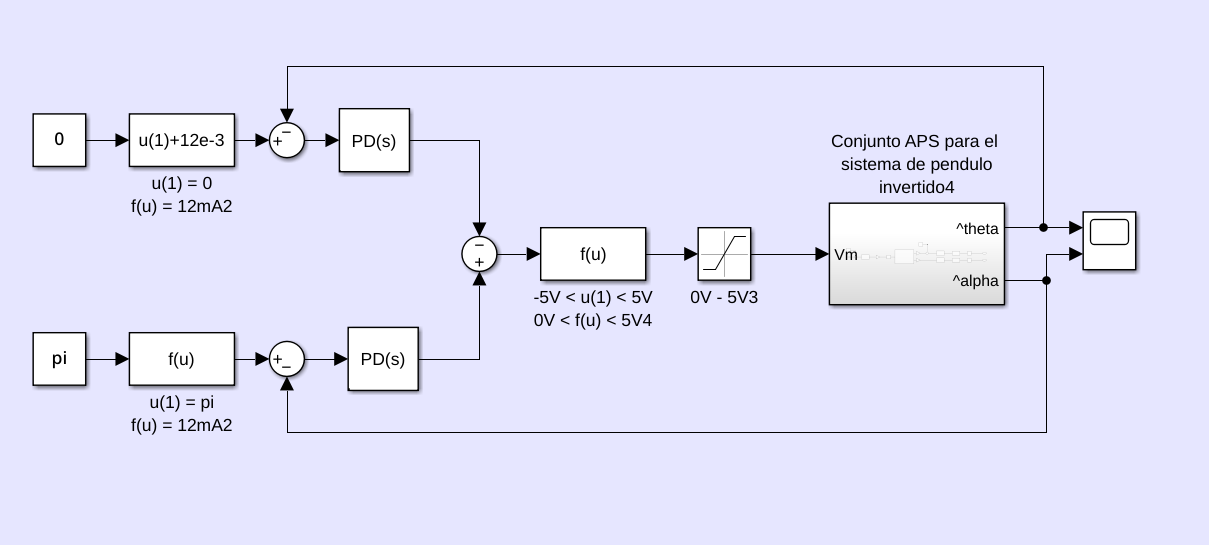
\includegraphics[width = 0.8\linewidth]{figs/lc.png}
    \caption{Esquema de control para péndulo invertido rotatorio}
    \label{db}
\end{figure}

Por tanto, la variable manipulada se compone como una combinación lineal de la respuesta de dos controladores
distintos, $C_{\theta}(s)$ y $C_{\alpha}(s)$, cada uno para un ángulo diferente.
Como la señal realimentada es de corriente, se tuvo que normalizar los 
valores deseados.
Y también, como se restan las salidas de ambo PIDs cuyas salidas están saturadas en el rango
especificado, se tuvo que normalizar nuevamente. 
Estas relaciones vienen dadas por \eqref{lcNorm}.
\begin{equation}
    \begin{aligned}
        \widetilde{V_m}(t) &= \frac{1}{2}(V_m^\alpha - V_m^\theta) + 2.5\label{lcNorm}\\
        \Delta\alpha^*(t) &= \frac{ \SI{12e-3}{}}{\pi}\Delta\alpha^*_{rad}\\
        \Delta\theta^*(t) &= \Delta\theta^*_{rad}+ \SI{12e-3}{}\\
    \end{aligned}
\end{equation}
\subsection{Sintonización de controladores}
Las funciones de transferencia $C_{\theta}(s)$ y $C_{\alpha}(s)$ se implementaron por medio de controladores
de la familia PID tipo paralelo.
Al ser $P_{\theta}(s)$ integrante y $P_{\alpha}(s)$ inestable, se escogió usar controladores tipo PD, con filtro derivativo.
Estos controladores aseguraron cero error en estado estacionario alrededor del punto de operación escogido, el cual
corresponde a un punto de estabilidad del mismo.
Por tanto, la forma general de estos controladores es \eqref{PDs}.
\begin{equation}
    \begin{aligned}
        C(s) = K_p + \frac{K_ds}{ \frac{s}{K_f} + 1}\label{PDs}\\
    \end{aligned}
\end{equation}
A pesar de que \eqref{PDs} no sea la forma en la que se implementan esta familia de controladores en Simulink,
se escogió trabajar con esta topología, que previamente se ha trabajado en el programa de simulación PLECs, debido 
a comodidad, y no con la forma en que MATLAB lo trabaja.
Se sintonizaron ambos controladores de 3 formas diferentes:
\begin{itemize}
    \item LGR y sintonización empírica
    \item Optimización para servocontrol centrada en desempeño con respecto al IAE
    \item Optimización para servocontrol centrada en robustez con respecto al IAE
\end{itemize}
Para cada caso, primero se sintonizó $C_{\alpha}(s)$ y después $C_{\theta}(s)$.
La sintonización por LGR implicó la cancelación de los polos de las plantas por medio
de ceros del controlador.
Se tuvieron problemas con la ganancia negativa de $P_{\theta}(s)$ al realizar LGR, por lo que 
$C_{\theta}(s)$ se sintonizó empíricamente en este caso.
Los problemas de optimización que se plantearon para las últimas dos sintonizaciones se muestran
en \eqref{optimizacion}.

\begin{equation}
    \begin{aligned}
        \underset{K_p\,K_d\,K_f}{\text{min}}&IAE_{des}\label{optimizacion}\\
        \underset{K_p\,K_d\,K_f}{\text{min}}&IAE_{opt} \quad \text{s.t} \quad M_s = 1.1
    \end{aligned}
\end{equation}
Lo cual se aplicó para cada controlador.
Es decir, cuatro problemas de optimización, cada una con una función de costo, 
cuya forma general es \eqref{costo}.
\begin{equation}
    \begin{aligned}
        IAE = \int_0^t r(t) - y(t)\,dt\label{costo}
    \end{aligned}
\end{equation}
Por efectos de hacer el reporte lo más al grano posible, no se pondrán todas 
las ecuaciones que implica lo anterior.
Las optimizaciones se realizaron simulando el diagrama de bloques de Simulink del sistema a lazo cerrado
dentro de la función de costo que \texttt{fmincon} y \texttt{fminsearch} utiliza.
Se usaron los parámetros obtenidos a partir de LGR y la sintonización empírica como parámetros de partida
para las optimizaciones que se realizaron.
Los parámetros obtenidos se muestran en el \hyperref[parametros]{Cuadro ~\ref{parametros}}.

\begin{table}
\centering
\begin{tabular}{lcccccc}
\toprule
& \multicolumn{2}{c}{LGR/Empírico} & \multicolumn{2}{c}{Opt Desempeño} & \multicolumn{2}{c}{Opt Robustez} \\
\cmidrule(lr){2-7} 
& $C_{\alpha}(s)$ & $C_{\theta}(s)$ & $C_{\alpha}(s)$ & $C_{\theta}(s)$ & $C_{\alpha}(s)$ & $C_{\theta}(s)$ \\
\midrule
$K_p$ & \SI{3001}{}  & 500   & 2671.475  & 788.703   &  669.650  &   3722.750\\
$K_d$ & \SI{145.704}{}  & 200   & 212.090   & 320.988   &  239.262  &   154.931\\
$K_f$ & \SI{7524.45}{} & 2000   & 2176.104  & 503.486   &  2389.741 &   6838.319\\
\bottomrule
\end{tabular}
\caption{Parámetros de los controladores para diferentes métodos de sintonización.}
\label{parametros}
\end{table}

\section{Validación del sistema de control}
En \href{https://youtu.be/ISYTeRPDpHw?si=HoDpNC0XWb7yOUdD}{este video} se muestra la 
validación del sistema de control.
A pesar de que se debían de colocar las curvas dinámicas del sistema, se me imposibilitó debido
a que no encuentro por ningún lado el archivo de Simulink que se muestra en el video. 
Sin embargo, esto permite que el reporte sea aun más al grano, 
ya que puede visualizar las gráficas de la validación del sistema de control en conjunto
con la simulación de Simscape que muestra la respuesta física del péndulo.
Los eventos que suceden en la simulación se muestran a continuación.
\begin{itemize}
    \item $t\in[0,\,3]\,\text{s}$: Se parte la simulación con el péndulo inclinado $30^\circ$ con respecto al eje $z$.
        El lazo de control centrado a desempeño es el que se asienta más rápido de los tres, pero tiene la respuesta más agresiva,
        seguida por el lazo de control con rltool, y por último el lazo de control centrado en robustez, siendo este el que dura más 
        en asentarse.
        Esto es esperado, debido a que existe un compromismo entre robustez y desempeño, por tanto es normal que este último lazo
        dure varios segundos más en asentarse en comparación a los otros dos.

    \item $t\in[3,\,7.5]\,\text{s}$: Se aplica un cambio escalón en la perturbación.
        Menos de medio segundo después, se quita el efecto de la perturbación.
        Esto se debe a que, si $\Delta \widehat{\alpha}(t)$ se sale del punto de operación
        establecido en el \hyperref[t1]{Cuadro 1}, el sistema se desestabiliza y es imposible
        recuperar el control del mismo.
        Como $\sum \tau = I\alpha$, donde $\alpha$ denota aceleración angular e $I$ momento de inercia, es necesario desaplicar
        el torque para que $\Delta \widehat{\alpha}(t)$ no llegue a un punto crítico en donde se desestabilice el
        sistema.
        Como los 3 lazos de control se sintonizaron para servocontrol, la respuesta entre el lazo de rltool y el lazo centrado en desempeño
        es muy similar. Por otro lado, se observan oscilaciones nuevamente en el lazo centrado en robustez, debido a que una menor sensibilidad
        provoca un peor desempeño, lo cual se ve reflejado en un mayor tiempo de asentamiento y la presencia de sobrepasos más prolongados.
\end{itemize}

Note que los controladores son tipo PD, por lo que no tiene sentido hablar sobre anti-windup para el sistema de control
diseñado, ya que esto solo se implementa en controladores con modo integral.
